\section{Probability and Statistics}
A great deal of the machine learning principles are based on concepts from probability theory and statistics. As we will encounter later on, we are often facing a scenario where for the task in hand we:
\begin{itemize}
	\item Define some parameter (or set of parameters) of interest.
	\item Define some objective function that depends on this parameter. 
	\item Have some data relevant to the task, from which we try to \textbf{estimate} the \textbf{parameter} by optimizing the \textbf{objective function}.
\end{itemize}

~\\Consider the following task. We are preparing the traditional ``Introduction to Machine Learning Hackathon`` and expecting 500 hungry students. For this event we want to order enough pizzas for all the participants. How should we know how many pizzas to order? Let us denote the average number of pizza slices each participant would like to eat by $\mu$. In statistics, this average is called the \textit{population mean}, meaning simply that it refers to an average over the whole group which is under consideration. In this case, all $N$ participants.

~\\Then, a reasonable guess for the number of pizza slices we should order is $X=N \times\mu$. As we do not know $\mu$, and it would take too long to ask each of the participants how many pizza slices they would like to have, we must come up with some way to \textbf{estimate} a value of $\mu$. To do so, let us \textit{sample independently} participants: we randomly choose one, call and ask how many pizza slices they would like to eat. We write the answer down as $x_1$. We then randomly call another one (which could accidentally be the same one) and write the second answer as $x_2$. We continue $m$ times. Now, to estimate the population mean, $\mu$, we use the average of the answers acquired. In statistics this is referred to as the \textit{sample mean} and is given by
$$\widehat{\mu} \equiv \frac{1}{m}\sum_{i=1}^{m}x_i.$$
Namely, the empirical average of the parameter in question. Finally, we \textit{predict} that we will need $T= N \times \widehat{\mu}$ pizza slices. The $\widehat{\mu}$ (hat) symbol indicates that this is an estimator of the parameter $\mu$.

~\\Another question is how many participants should we contact? Intuitively, if we ask a very small set of participants our estimation of $\widehat{\mu}$ (and therefore our prediction of $T$ would be very wrong. As we increase the number of participants asked, the \textit{sample size}, we will get a more accurate estimation of $\widehat{\mu}$. To answer how accurate of an estimation, let us suppose that we know the true value of $\mu$. Then we should look at the difference between our estimation and the true value, and how it changes as $m$ changes. We can then choose an accuracy parameter $\eps > 0$ and require that $\left|\widehat{\mu} - \mu\right|\leq \eps$. By solving for $m$ we will get a bound on the number of participants we should ask.


\subsection{Fundamental Definitions}
\subsubsection{Probability Space}
The basic object in probability theory is that of a \emph{probability space} which consists of two ingredients: the \textit{sample space} and the \textit{probability function}.
\begin{definition}
A \textit{sample space} $\Omega$ is a set that contains all possible outcomes. $\omega\in\Omega$ denotes a single outcome.
\end{definition}

For exmple the probability space of $m$ coin tosses can be defined as $\Omega=\left\{ H,T\right\}^m $ or the probability space of coin tosses until heads comes up can be defined as $\Omega=\left\{ T^{n-1}H:n\in\N\right\} $. We can also define more complex probability spaces such as the height, weight, blood pressure and sex of patients with a medical condition, as well as the success or failure of an experimental drug: $\Omega=[0,\infty)\times [0,\infty) \times[0,\infty) \times \{M,F\}\times \{Yes,No\} $. As we will see, we often model machine learning tasks with some probability space (even if we do not explicitly define it).

\begin{definition}
An \textit{event} $A$ is any subset of possible outcomes, $A\subseteq\Omega$.
\end{definition}

\begin{definition}
	A \textit{probability space} is a tuple \footnote{For our needs this simple and intuitive definition is sufficient, though, richer definitions exist.} $(\Omega, \Dc)$ where $\Omega$ is a \emph{sample space} and $\Dc:2^{\Omega}\rightarrow\R$ is a probability function such that
	\begin{enumerate}
		\item $\Dc(\Omega)=1$
		\item for all $\omega\in\Omega, \Dc(\omega)\in[0,1]$
		\item for all $A,B\subseteq\Omega$ such that $A\cap B=\emptyset,$ we have $\Dc(A \cup B)=\Dc(A)+\Dc(B).$
	\end{enumerate}
\end{definition}

\begin{example}
	Suppose we throw two fair dice, then $\Omega=\left\{ 1,\dots,6\right\} ^{2}$ and $\Dc\left(\left(i,j\right)\right)=\frac{1}{36}$
\end{example}


\begin{claim}
	For all $A,B\subseteq\Omega$: $\Dc(A\cup B)=\Dc(A)+\Dc(B)-\Dc(A\cap B)$
\end{claim}
\begin{proof}
Let us notice that for both events $A,B$ it holds that:
$$
\begin{array}{c}
A=(A\setminus B)\cup(A\cap B)\\
B=(B\setminus A)\cup(A\cap B)
\end{array}
$$
and that $A\cup B=(A\setminus B)\cup(B\setminus A)\cup(A\cap B)$. Therefore
$$\begin{array}{ccl}
\Dc(A\cup B) & = & \Dc(A\setminus B)+\Dc(B\setminus A)+\Dc(A\cap B)\\
&=&\Dc(A)-\Dc(A\cap B)+\Dc(B) -  \cancel{\Dc(A\cap B)}  + \cancel{\Dc(A\cap B)} 
\end{array}$$
\end{proof}

\begin{definition}
Events $A,B\subseteq\Omega$ are said to be \textit{independent} if the occurrence of one does not affect the probability of occurrence of the other, namely: $$\Dc(A\cap B) =\Dc(A)\cdot\Dc(B)$$
\end{definition}

\begin{exercise}
Show that if $A$ and $B$ are independent then $A$ and $B^c$ ($\Omega\setminus B$) are also independent.
\end{exercise}
\begin{proof}
As $\Dc(A)=\Dc(A\cap B)+\Dc(A\cap B^c)$ Then $\Dc(A\cap B^c)=\Dc(A)(1-\Dc(B))=\Dc(A)\cdot\Dc(B^c)$
\end{proof}

\begin{theorem}[The union bound] Let $(\Omega, \Dc)$ be a probability space. The probability function is \emph{sub-additive}, i.e., for any sequence $\left(A_k\right)$ of events,
	\[
	\Dc\left(\cup_{k=1}^\infty A_k\right) \le \sum_{k=1} ^\infty \Dc\left(A_k\right)
	\]
\end{theorem}
\begin{proof}
Let $B_1=A_1$. For each $k \in \{2,3,\ldots\}$, let $B_k = A_k\setminus \cup_{i=1}^{k-1} A_i$. Note that the $B_1,\ldots,B_k$ are disjoint, and that $\cup_{i=1}^k A_i=\cup_{i=1}^k B_i$. Also, since $B_k\subseteq A_k$, $\Dc(B_k) \le \Dc(A_k)$ for every $k \in \N$. It follows that:
	\[
	\Dc\left(\cup_{k=1}^\infty A_k\right) = \Dc\left(\cup_{k=1}^\infty B_k\right) = \sum_{k=1}
	^\infty \Dc\left(B_k\right) \le \sum_{k=1}
	^\infty \Dc\left(A_k\right)
	\]
\end{proof}


\subsubsection{Random Variables}

So far we have asked questions like: does an event happen or not and what is the probability of the event. How would we be able to model different questions such as, "how much". For example, suppose if a coin flip turns head we get a dollar, we can ask how many dollars would we get after 3 rounds?  

~\\In order to answer this question, we should identify the sample space, which is $$\Omega=\left\{HHH,HHT,HTH,THH,HTT,THT,TTH,TTT\right\}$$ Then, we would need to define a reward function that will quantify ones's profit for each outcome of the experiment ($\omega\in \Omega$): $X\left(HHH\right)=3,\, X\left(HHT\right)=2$ and so on. This quantifying function $X$ is called a \textit{random variable} (RV).

\begin{definition}
Given a probability space $\left(\Omega,\Dc\right)$, a real-valued \textit{random variable (RV)} is a function $X:\Omega\rightarrow\R$.
\end{definition}

\begin{definition}
Let $\Omega$ be a discrete probability space and $X$ a random variable over $\Omega$. The \textbf{\textit{probability
		mass function (PMF)}} of $X$ is defined as:
\[
\Dc\left(\left\{ X=x\right\} \right)=\sum_{\omega:X\left(\omega\right)=x}\Dc\left(\omega\right)
\]
\end{definition}

Instead of writing $\Dc\left(\left\{ X=x\right\} \right)$ we can simplify notation as $\Dc_X\left(\left\{ x\right\} \right)$, and further simply as $\Dc\left(x\right)$. This simplified notation, omitting any reference to the random variable, is useful when the context is clear and we shall use it often. This omission is similar to saying, for example,  "the probability of $\left(H,T\right)$ is 1/4" instead of "the probability of getting $\left(H,T\right)$ by tossing a fair coin twice is 1/4".

\begin{example}
A fair coin is tossed twice. The probability space is given by $\Omega=\left\{ T,H\right\} ^{2}$. As this is a fair coin then $\forall \omega\in\Omega \,\, \Dc\left(\omega\right)=\frac{1}{4}$. Let $X$ denote the number of heads obtained in each outcome ($\omega$). The possible values of $X$ are 0, 1, and 2. The probability of each value is
	\[
	\Dc\left(x\right)=\begin{cases}
		\frac{1}{4} & x=0,2\\
		\frac{1}{2} & x=1\\
		0 & \mbox{else}
	\end{cases}
	\]
\end{example}


\begin{definition}
Let $\Omega$ be a continuous probability space and $X$ a random variable over $\Omega$. We say that $X$ is a \textit{continuous random variable} if there exists $f\left(x\right)\ge 0$ so that we can write, for every $D\subset\R$
\[
\Dc\left(X\in D\right)=\int_{D}f\left(x\right)dx
\]

The function $f$ is called the \textbf{\textit{probability density function }} \textbf{(PDF)} of $X$.
\end{definition}

In particular, this means that for any $a,b\in \R$, where $a\leq b$:
\[
\Dc\left(X\in\left[a,b\right]\right)=\int_{a}^{b}f\left(x\right)dx
\]

As before, $f$ should actually be denoted by $f_X\left(x\right)$ to emphasize that it characterizes the random variable $X$, but often the subscript $X$ is omitted. In this course we assume that $f(x)$ is a regular function and therefore the probability mass function for a single point is 0: $\Dc\left(X=a\right)=\int_{a}^{a}f\left(x\right)dx=0$ for any $a\in\R$. Note that the probability density function satisfies that
\begin{itemize}
	\item $f\left(x\right)\ge0$
	\item $\int_{-\infty}^{\infty}f\left(x\right)dx=1$
	\item $f\left(x\right)$ is a probability \emph{density}, not a probability. For example, it could be that $f\left(x\right)>1$.
\end{itemize}

\subsubsection{Mean and Variance}
When dealing with random variables (and later on with distributions) we are often interested in different measures of these random variables. The two most common and widely used measures are the mean (expected value) and variance.

\begin{definition}
The \textbf{\textit{expected value}} of a random variable $X$ is
$$ \E  \left[X\right]\coloneqq\sum_{x\in\mathcal{X}}x\Dc\left(x\right)\qquad\mbox{or}\qquad \E \left[X\right]=\int_{-\infty}^{\infty}xf\left(x\right)dx	$$
\end{definition}

\begin{claim}
Let $X,Y$ be two random variable with finite expected values $\E\left[X\right],\E\left[Y\right]$. Then:
\begin{itemize}
	\item Linearity of expectation: $\E \left[aX+Y\right]=a\E \left[X\right]+\E \left[Y\right]$.
	\item Expectation of function of random variable (Law of the unconscious statistician): $\E \left[g\left(X\right)\right]=\sum g\left(x\right)\Dc\left(x\right)$.
	\item If $X$ and $Y$ are independent then:  $\E \left[XY\right]=\E \left[X\right]\E \left[Y\right]$.
	\item If $X\leq Y$ then $\E\left[X\right]\leq \E\left[Y\right]$.
\end{itemize}
\end{claim}

\begin{definition}
Let $X$ be a random variable with $\E \left[X\right]$, then the \textbf{\textit{variance}} of $X$ is
$$Var\left(X\right)\coloneqq\E \left[\left(X-\E\left[X\right]\right)^{2}\right]$$
The \textbf{\textit{standard deviation}} of $X$ is defined as $\sigma\coloneqq\sqrt{Var\left(X\right)}$.
\end{definition}
\begin{claim}
Let $X,Y$ be two random variables with finate expected values and variances. Then:
\begin{itemize}
	\item $Var\left(X\right)=\E \left[X^{2}\right] - (\E \left[X\right])^{2}$
	\item For scalars $a,b\in\R$, $Var\left(aX+b\right)=a^{2}Var\left(X\right)$
	\item The variance of $X$ is non-negative: $Var(X)\geq0$. Equality holds when $Var(X)=0\,\iff\,X$ is a constant.
	\item $\begin{array}{ccl}Var\left(X+Y\right)&=&\E \left[\left(X+Y-\E (X)-\E (Y)\right)^{2}\right]\\ &=& Var(X)+Var(Y)+2\E \left[\left(X-\E [X]\right)\left(Y-\E [Y]\right)\right]\end{array}$
	\item If $X_{1},\dots,X_{n}$ are independent then $V\left(\sum X_{i}\right)=\sum V\left(X_{i}\right)$
\end{itemize}
\end{claim}

\begin{definition}
The \textbf{\textit{covariance}} (joint variability) of $X$ and $Y$ is the expected value of the product of their deviations from the expected values
$$
Cov\left(X,Y\right) \coloneqq \left[\left(X-\E [X]\right)\left(Y-\E [Y]\right)\right]=\E \left[XY\right]-\E [X]\E [Y]
$$
The covariance is also denoted as $\sigma\left(X,Y\right)$ or $\sigma_{XY}$.
\end{definition}

\begin{claim}
Let $X,Y$ be two random variables with finite expectation and variance. Then:
\begin{itemize}
	\item Symmetry: $Cov\left(X,Y\right)=Cov\left(Y,X \right)$.
	\item For scalars $a,b,c,d\in\R$, $Cov\left(aX+b,cY+d \right) = a \cdot c \cdot Cov \left(X,Y \right)$
	\item $Cov\left(X,X\right)=Var\left(X\right)$
\end{itemize}
\end{claim}

Note the different meaning implied by the above definitions: The variance measures the variation of a single random variable (like the height of a person in a population), whereas covariance is a measure of how much two random variables (like the height and weight) vary together.

\begin{example}
Let $Z$ be a random variable such that $P\left(Z=1\right) = p, P\left(Z=0\right) = 1-p$. The variance of $Z$ is: $Var\left[Z\right] = \E \left[Z^2\right] - \left(\E \left[Z\right]\right)^2 = p-p^2=p\left(1-p\right)$.
\end{example}

\begin{exercise}
Let $X\sim Unif\left(\left[a,b\right]\right)$ for $a,b\in\R$. Calculate the expectation and variance of $X$.
\end{exercise}
\begin{proof}
$$\begin{array}{ccl}
\E \left[X\right]  &=&  \frac{1}{b-a}\int_{a}^{b} xdx=\frac{b+a}{2}\\
\E \left[X^{2}\right]  &=& \frac{1}{b-a}\int_{a}^{b}x^2 dx =\frac{b^{2}+ab+a^{2}}{3}\\ \\
Var\left(X\right)  &=&  \frac{b^{2}+ab+a^{2}}{3}-\frac{\left(b+a\right)^{2}}{4}=\frac{\left(b-a\right)^{2}}{12}
\end{array}$$
\end{proof}



\subsection{A Little Statistics: Mean and Variance Estimation}
The focus of this book is {\em Statistical} Machine Learning.  When we study {\em Probability} we assume a known distribution and calculate probability of events of interest. When we study {\em Statistics} we turn the question on its head: using samples from an unknown probability distribution, we try to {\em estimate} or {\em test} properties of the unknown distribution. Recall the pizza slices example: we were interested in finding out how many pizza slices the participants will eat. We did not know what is the distribution of number of pizza slices participants eat. Given {\em samples} that were drawn from this unknown distribution, we attempted to {\em estimate}  the distribution's mean. Let us formulate what we have done above and estimate both the expected value and the variance.

~\\Let $X$ be a random variable and let $\Dc \left(x\right)$ be its (unknown) distribution. Let $X_1,\ldots,X_m\overset{i.i.d}{\sim} D(x)$ be $m$ random variables of this distribution. The $i.i.d$ denotes these are \emph{independent and identically distributed} random variables. We are given \emph{data samples}: $x_1,\ldots,x_m$, where each $x_i$ is a {\em number} obtained by sampling $X_i$. In statistics, $\E\left[X\right]$ is called the {\em population} mean - "population" added to emphasize that it is the mean of the unknown distribution, and not of the observed data. Similarly, $Var\left(X\right)$ is called the \textit{population variance}.

~\\There are many ways to estimate $\E\left[\right]$ and $Var\left(X\right)$ based on those $m$ samples, and each one is called an \textit{estimator} (that is, the function that estimates the value of some parameter of a random variable). Throughout this book we are going to use different estimators for different tasks. For the case of sample mean and variance we will use:
\begin{itemize}
	\item \textbf{\textit{Sample mean}} (an estimator for the population mean) $$ \widehat{\mu}_X = \frac{1}{m} \sum_{i=1}^m x_i$$
	\item \textbf{\textit{Sample variance}} (an estimator for the population variance)$$\widehat{\sigma}_X^2 = \frac{1}{m-1} \sum_{i=1}^m (x_i-\widehat{\mu}_X)^2$$
\end{itemize}

As meantioned before, whenever the context is clear, we will omit the subscript $X$ and write $\widehat{\mu}$ and $\widehat{\sigma}^2$ instead of $\widehat{\mu}_X$ and $\widehat{\sigma}_X^2$. Note that the sample variance is somewhat different from the variance of the $x_i$'s because of the division by $m-1$ instead of $m$. The difference between the two will be explained later on in the book.

\begin{exercise}
Let $X$ be some random variable. Show that the expected values of the samples mean and sample variance estimators equals to the true parameters they estimate. That is their expectation is the population mean and population variance.\\

\textbf{Solution}. Taking the expectation value of the sample mean one gets
$$
\E\left(\widehat{\mu}_X\right) = \E\left(\frac{1}{m} \sum_{i=1}^m x_i\right) = \frac{1}{m} \sum_{i=1}^m \E\left(x_i\right) = \E\left(X\right) \frac{1}{m} \sum_{i=1}^m 1 =  \E\left(X\right)= \mu_X
$$ 
where we used the linearity property of the expectation and that the samples are $i.i.d$. Taking the expectation value of the sample variance one gets
$$
\begin{array}{ccl}
\E\left(\widehat{\sigma}_X^2\right) & = & \frac{1}{m-1} \sum_{i=1}^m \E\left((x_i-\widehat{\mu}_X)^2\right)\\
& = & \frac{1}{m-1} \sum_{i=1}^m \E\left(x_i^2-2x_i\frac{1}{m} \sum_{j=1}^m x_j+\frac{1}{m^2} \sum_{i,j=1}^m x_ix_j\right)
\end{array}
$$
The $X_i$'s are i.i.d which implies that  $\E\left(x_i\right)=\E\left(X\right)$ and $\E\left(x_i^2\right)=\E\left(X^2\right)$ for every $i$, as well as that   $\E\left(x_ix_j\right)=\E^2\left(X\right)=\mu^2_X$ for every  $i\neq j$. Substituting into the above sums we obtain that:
$$
\E\left(\widehat{\sigma}_X^2\right) =\E\left(X^2\right) -\E^2\left(X\right)=Var\left(X\right)= \sigma^2_X
$$
\end{exercise}


\begin{definition}
Let $\widehat{\theta}$ be an estimator of $\theta$. The \textit{bias} of $\widehat{\theta}$ is the expected deviation between $\theta$ and the estimator: $B\left(\widehat{\theta}\right)\coloneqq\E\left[\widehat{\theta}\right]-\theta$. $\widehat{\theta}$ is said to be \textit{unbiased} if $B\left(\widehat{\theta}\right)=0$.
\end{definition}

From what we have seen in the above exercise,  $\widehat{\mu}_X$ is an unbiased estimator of the population mean, $\mu_X$, and $\widehat{\sigma}_X^2$ is an unbiased estimator of the population variance $\sigma^2_X$. If we calculate the expected variance of the $x_i$'s using $\frac{1}{m} \sum_{i=1}^m (x_i-\hat{\mu}_X)^2$, we will see that we do not get the value $\sigma^2_X$, but rather is $\frac{m-1}{m}\sigma^2_X$. Therefore this estimator is a \textit{biased} estimator of $\sigma^2_X$. 

\begin{remark}
Biased estimator, though there expectation is not the true value of the parameters can be useful in different cases. Therefore, we would sometimes use biased estimators and sometimes unbiased estimators.
\end{remark}

\subsection{Multivariate Probabilities}
Up to now, we only dealt with random variables taking a single value. In many machine learning applications however, we often face a situation where we have multiple properties we would like to use in order to perform prediction. To do that we consider multivariate random variables and multivariate distributions.

\begin{definition}[Random vector]
A  (column)	\textbf{\textit{random vector}}: $X\coloneqq \left(X_1, \dots, X_d\right)^\top$, is a finite collection of random variables, denoted $X_1, \dots, X_d$, defined on a common probability space $(\Omega, \Dc)$.
\end{definition}

\begin{definition}[Joint distribution]
Given random variables $X_1, \dots, X_d$, that are defined on a probability space, the joint probability distribution for $X_1, \dots, X_d$ is a probability distribution that gives the probability that each of $X_1, \dots, X_d$ falls in any particular range (for continuous RVs) or discrete set (for discrete RVs) of values specified for that variable.
\end{definition}

\begin{definition}[Joint PDF of a random vector]
Two random variables $X_1$ and $X_2$ are \textbf{\textit{jointly continuous}} if there exists a non-negative function $f_{X_1,X_2}: \R^2\to\R $, such that, for any set $A \in\R ^2$, it holsd that $$\Dc\left( (X,Y) \in A \right) = \int_A f_{X_1,X_2}\left(x_1, x_2\right) dx_1 dx_2$$

The function $f_{X_1,X_2}$ is called the \textbf{\textit{joint probability density function (JPDF)}} of $X_1$ and $X_2$. Often, if the context is clear, one omits the subscripts of $f$ and simply writes  $ f\left(x_1, x_2\right)$.
\end{definition}

Given $X \coloneqq (X_1, \dots, X_d)^\top$, each of the scalar random variables $X_1, \dots, X_d$ can be characterized by its PDF. However, unless the scalar RV's are mutually independent, the PDF of each coordinate of a random vector does not completely describe the probabilistic behavior of the whole vector. For instance, the behavior of the random vectors $X = \left(X_1, X_2\right)$ and $\tilde{X} = \left(X_1, X_1\right)$ is drastically different even if $X_1$ and $X_2$  have an identical PDF. Consider for example, $X_1, X_2 \sim Unif([-a, a])$ and $X_2 = - X_1$ and compare the probability to find $X$ in the square $[0,1]\times [0,1]$ to that of finding $\tilde{X}$ in the same square.

	
\subsubsection{Normal Distribution}
As an example of random vectors, we now consider specific family of distributions - the Multivariate Normal (also called Multivariate Gaussian) Distributions. Due to different limit theories, such as the Central Limit Theorem, and due to nice mathematical properties of this distribution, it is often used to model different probabilistic scenarios.

\begin{definition}[(Univariate) Normal Distribution] \label{def: UVN}
A random variable $x$ has a \textbf{\textit{normal distribution}} with expectation $\mu$ and variance $\sigma^2$ if it has a PDF of the form:
	$$f\left(x\right) = \frac{1}{\sqrt{2\pi\sigma^2} } \exp^{ -\frac{1}{2\sigma^2} \left(x-\mu\right)^2 } $$
In this case we write: $x\sim\Nc(\mu,\sigma^2)$
	
\end{definition}
\begin{definition}[Multivariate Normal Distribution] \label{def: MVN}
A random vector $\x\in\R^d$ has a \textbf{\textit{multivariate normal distribution}} with expectation $\mu$ and covariance matrix (see definition below) $\Sigma$ if it has a joint PDF of the form: $$f\left(\x\right)=\frac{1}{\sqrt{\left(2\pi\right)^{d}\left|\Sigma\right|}}\exp\left\{ -\frac{1}{2}{\left(\x-\mu\right)^{\top}\Sigma^{-1}\left(\x-\mu\right)}\right\} $$
In this case we write: $\x\sim\Nc(\mu,\Sigma)$
\end{definition}

\begin{figure}[h!]
	\centering
	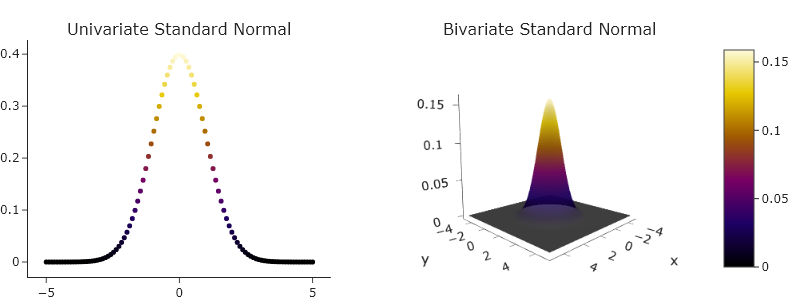
\includegraphics[width=0.9\textwidth]{chapters/mathematical.basis/figures/normal_distributions.png}
	\caption{Uni- and bivariate normal distributions. \GitChapterOneExamples}
\end{figure}

Observe that definition \ref{def: MVN} is generalization of \ref{def: UVN}, i.e. when $d = 1$ both definitions are same. Often, we are interested only in how one of the variates distributes, without the influence of the rest. For example, suppose we have joint probability function of the variables ``height`` and ``weight`` but we are interested in how the ``height`` distributes. To do so we would like to integrate out the ``weight`` variable. This leads to the following definition:

\begin{definition}
The \textbf{\textit{Marginal distribution}} of a subset if a collection of random variables with a joint probability distribution, is the probability distribution of the variables in the set: $$f\left(\x\right)=\int_{\y}f\left(\x,\y\right)d\y$$
\end{definition}
where the $\mathbf{y}$ integration is over all the random variables not in $\x$.

\begin{exercise}[Marginal of Bivariate Normal]
Let $\x\sim \Nc\left(\mu,\Sigma\right)$ where $\x\in\R^2, \mu=\left(\mu_1,\mu_2\right)^\top$ and $\Sigma=\left[\begin{array}{cc}\sigma_1^2&0\\0&\sigma_2^2\end{array}\right]$Find the PDF of the marginal distribution of $x_1$.

~\\Observe that we can write the PDF as follows:
$$
\begin{array}{ccl}
	f\left(\x\right) & = & \frac{1}{\sqrt{\left(2\pi\right)^{2}\left|\Sigma\right|}}\exp\left(-\frac{1}{2}\left(\x-\mu\right)^{\top}\Sigma^{-1}\left(\x-\mu\right)\right)\\
	& = & \frac{1}{\sqrt{\left(2\pi\right)^{2}\sigma_{1}^{2}\sigma_{2}^{2}}}\exp\left(-\frac{1}{2}\left[\begin{array}{c}
		x_{1}-\mu_{1}\\
		x_{2}-\mu_{2}
	\end{array}\right]\left[\begin{array}{c}
		\begin{array}{cc}
			\sigma_{1}^{-2} & 0\\
			0 & \sigma_{2}^{-2}
	\end{array}\end{array}\right]\left[\begin{array}{cc}
		x_{1}-\mu_{1} & x_{1}-\mu_{1}\end{array}\right]\right)\\
	& = & \frac{1}{\sqrt{\left(2\pi\right)^{2}\sigma_{1}^{2}\sigma_{2}^{2}}}\exp\left(-\frac{1}{2}\left(\frac{x_{1}-\mu_{1}}{\sigma_{1}}\right)^{2}\left(\frac{x_{2}-\mu_{2}}{\sigma_{2}}\right)^{2}\right)\\
	& = & \frac{1}{\sqrt{\left(2\pi\right)^{2}\sigma_{1}^{2}}}\exp\left(-\frac{1}{2}\left(\frac{x_{1}-\mu_{1}}{\sigma_{1}}\right)^{2}\right)\cdot\frac{1}{\sqrt{\left(2\pi\right)^{2}\sigma_{2}^{2}}}\exp\left(-\frac{1}{2}\left(\frac{x_{2}-\mu_{2}}{\sigma_{2}}\right)^{2}\right)
\end{array}
$$

Using the definition of the marginal distribution:
$$
\begin{array}{ccl}
	f\left(x_{1}\right) & = & \intop_{-\infty}^{\infty}f\left(x_{1,}x_{2}\right)dx_{2}\\
	& = & \intop_{-\infty}^{\infty}\frac{1}{\sqrt{\left(2\pi\right)^{2}\sigma_{1}^{2}}}\exp\left(-\frac{1}{2}\left(\frac{x_{1}-\mu_{1}}{\sigma_{1}}\right)^{2}\right)\cdot\frac{1}{\sqrt{\left(2\pi\right)^{2}\sigma_{2}^{2}}}\exp\left(-\frac{1}{2}\left(\frac{x_{2}-\mu_{2}}{\sigma_{2}}\right)^{2}\right)dx_{2}\\
	& = & \frac{1}{\sqrt{\left(2\pi\right)^{2}\sigma_{1}^{2}}}\exp\left(-\frac{1}{2}\left(\frac{x_{1}-\mu_{1}}{\sigma_{1}}\right)^{2}\right)\cdot\intop_{-\infty}^{\infty}\frac{1}{\sqrt{\left(2\pi\right)^{2}\sigma_{2}^{2}}}\exp\left(-\frac{1}{2}\left(\frac{x_{2}-\mu_{2}}{\sigma_{2}}\right)^{2}\right)dx_{2}
\end{array}
$$
Notice that now we integrate a function of a uni-variate Gaussian for all values $x_2\in\left(-\infty,+\infty\right)$. Therefore this integral equals to $1$ and we are left with:
$$ f\left(x_1\right) = \frac{1}{\sqrt{\left(2\pi\right)^{2}\sigma_{1}^{2}}}\exp\left(-\frac{1}{2}\left(\frac{x_{1}-\mu_{1}}{\sigma_{1}}\right)^{2}\right) $$
Which by definition \ref{def: UVN} is a univariate Gaussian of the form $x_1\sim\Nc\left(\mu_1,\sigma_1^2\right)$.
\end{exercise}



\subsubsection{Covariance Matrix}
Unlike the univariate case, when dealing with a multivariate distribution the variance is a matrix rather than a vector.

\begin{definition}[Covariance Matrix]
Let $ \X \coloneqq\left(X_{1},X_{2},...,X_d\right)^\top$ be a random vector. The  {\em Covariance Matrix} $\Sigma$ is the $d \times d$ matrix whose $\left(i,j\right)$ entry is the covariance $\Sigma_{ij}\coloneqq\sigma\left(X_i,X_j\right)$:

$$\Sigma\coloneqq\left(\begin{array}{ccc}
	\E\left[\left(X_{1}-\E\left[X_{1}\right]\right)\left(X_{1}-\E\left[X_{1}\right]\right)\right] & ... & \E\left[\left(X_{1}-\E\left[X_{1}\right]\right)\left(X_{d}-\E\left[X_{d}\right]\right)\right]\\
	\vdots & \ddots & \vdots\\
	\E\left[\left(X_{d}-\E\left[X_{d}\right]\right)\left(X_{1}-\E\left[X_{1}\right]\right)\right] & ... & \E\left[\left(X_{d}-\E\left[X_{d}\right]\right)\left(X_{d}-\E\left[X_{d}\right]\right)\right]
\end{array}\right)$$

\begin{itemize}
\item In matrix notation we can express the covariance matrix as: $$\Sigma\coloneqq\E\left[(X - {\E\left[X\right]} )({X} -{\E\left[X\right]} )^\top\right]$$
\item The diagonal elements of $\Sigma$ are $\sigma\left(X_i, X_i\right) \equiv \sigma^2 _{X_i} \equiv  Var\left(X_i\right)$. $Sigma$ is a symmetric positive semi-definite matrix.
\end{itemize}
\end{definition}


Back to statistics, let us consider how to estimate the covariance matrix based on a given sample. In this context, $\Sigma$ is called the {\em population covariance matrix}.
Let us start with the bi-variate case $d=2$. Consider a two-dimensional random vector $\X=\left(X_1,X_2\right)^\top$, where, for example, $X_1$ is the height of a person and $X_2$ is the weight.

~\\Taking a sample of $m$ people from the population, we equip the data elements with two indices, the first stands for person's designated number and the second for the feature (1 for height, 2 for weight). Therefore, the height samples are denoted by  $x_{1,1},\ldots,x_{1,m}$ and the corresponding weight samples are $x_{2,1},\ldots,x_{2,m}$. Note that we can write the data as a matrix $X\in\R^{m \times d}$ where $m$ is the {\em sample size} and $d$ is the dimension (number of random variables). In our case, $d=2$ and
$$X = 
\left[\begin{array}{cc}
x_{1,1} &  x_{2,1} \\
\vdots & \vdots \\
x_{m,1} & x_{m,2}
\end{array}\right] = \left(\x_1,\ldots,\x_m\right)^\top
$$


\begin{definition}[Sample Covariance]
The unbiased estimator of the \textbf{\textit{sample covariance}} of the $i$'th and $j$'th random variables is given by:
$$\widehat{\sigma}\left(X_i, X_j\right) = \frac{1}{m-1} \sum^{m}_{k=1}{(x_{k,i}-\widehat{\mu}_i)(x_{k,j}-\widehat{\mu}_j)}$$
where $\widehat{\mu}_i$ is the sample mean of the random variable $X_i$.
\end{definition}
 
In particular, notice that for the case where $i=j$ we are left with the unbiased estimator previously seen. We can now define the sample covariance matrix $\widehat{\Sigma}$.

\begin{definition}[Sample Covariance Matrix]
Let $\X=\left(X_1,\ldots,X_d\right)^\top$ be a $d$-dimensional random vector and ket $\x_1,\ldots,\x_m\in\R^d$ be $m$ i.i.d samples of $\X$. The \textbf{\textit{sample covariance matrix}} is a square $d$-by-$d$ matrix $\widehat{\Sigma}$ such that $\widehat{\Sigma}_{i,j}=\widehat{\sigma}\left(X_{i},X_{j}\right)\quad i,j=1,\ldots,d$.

~\\In matrix notation the sample covariance matrix is given by:
$$ \widehat{\Sigma} \coloneqq \frac{1}{m-1} \sum^{m}_{i=1}\left(\x_i-\widehat{\mu}\right)\left(\x_i-\widehat{\mu}\right)^\top = \frac{1}{m}\X\X^\top $$
\end{definition}

\begin{exercise}
Let $\X=\left(\begin{array}{cc} 150 & 45\\ 170 & 74\\ 184 & 79 \end{array}\right)$ be samples of height and weight of 3 different people. Calculate the covariance matrix of the given sample.

~\\Let us begin with centering the data. That is, subtract the empirical mean from each sample
The sample mean is: $\widehat{\mu}=\left(168,66\right)^\top$, so:
$$\X_{centered}=\X - \left(\begin{array}{cc}
	168 & 66\\
	168 & 66\\
	168 & 66
\end{array}
\right)
=\left(\begin{array}{cc}
	150 & 45\\
	170 & 74\\
	184 & 79
\end{array}\right) - \left(\begin{array}{cc}
	168 & 66\\
	168 & 66\\
	168 & 66
\end{array}
\right)
=\left(\begin{array}{cc}
	-18 & -21\\
	2 & 8\\
	16 & 13
\end{array}\right)$$
Now, following the definition of the sample covariance matrix:
$$
\widehat{\Sigma} = \frac{1}{3-1}\X_{centered}\X_{centered}^\top=\left(\begin{array}{cc}
	292 & 301\\
	301 & 337
\end{array}\right)
$$
\end{exercise}


\subsubsection{Linear Transformations of the Data Set}
Let us look at how linear transformations affect the data set and as a result, the covariance matrix. Linear transformation can be of two types: scaling and rotating. Although we will now focus on the two-dimensional case, these results are easily generalized to higher dimensional data. The covariance matrix for two dimensions, $d=2$, is

$$\Sigma = \left( \begin{array}{ccc}  \sigma\left(X_1, X_1\right) & \sigma\left(X_1, X_2\right) \\  \sigma\left(X_2, X_1\right) & \sigma\left(X_2, X_2\right) \end{array} \right)$$

~\\We begin with a sample of points taken $i.i.d$ from a bi-variate Gaussian with a zero mean and equal variances $\sigma^2_{X_1}=\sigma^2_{X_2}\equiv  \sigma^2$ (\autoref{cov1}). In particular this means that $X_1$ and $X_2$ are uncorrelated and the covariance matrix $\Sigma$ is therefore of the form $\sigma^2 I_2$. In \autoref{cov1} we can indeed see that there is no apparent relation between a points $x$ coordinate and $y$ coordinate. When we calculate the sample covariance matrix, as the sample size $m$ increases, our estimation tends to $\widehat{\Sigma}=\sigma^2 I_2$.

\begin{figure}[H]
	\centering
	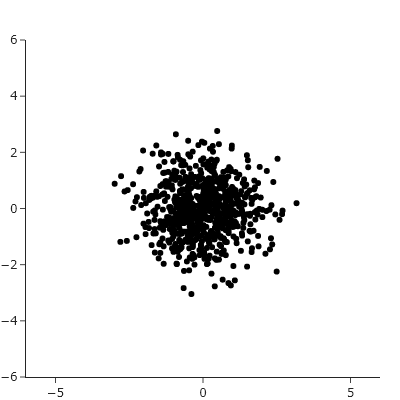
\includegraphics[width=0.35\textwidth]{chapters/mathematical.basis/figures/cov.png}
	\caption{Uncorrelated variables with identical variance. \GitChapterOneExamples}
	\label{cov1}
\end{figure}

Next, will us look at how linear transformations affect our data and the sample covariance matrix $\widehat{\Sigma}$ (\autoref{scaled_cov}). We start transforming our data by multiplication by a scaling matrix:

$$S = \left( \begin{array}{ccc}  s_{1} & 0 \\  0 & s_{2} \end{array} \right)$$

Notice how this transformation stretches (or shrinks) the $x_1$ and $x_2$ components of each sample by multiplying them by $s_{1}$ and $s_{2}$ respectively. In addition, as the scaling matrix is diagonal, the stretching of the $x$ axis is uncorrelated with that of the $y$ axis. The sample covariance matrix of the transformed data is:
$$\widehat{\Sigma}_{scaled}=\frac{1}{m-1}S\X\left(S\X\right)^\top=S\left(\frac{1}{m-1}\X\X^\top\right)S^\top=\left( \begin{array}{ccc}  (s_{1}\widehat{\sigma})^2 & 0 \\  0 & (s_{2}\widehat{\sigma})^2 \end{array} \right)$$.

\begin{figure}[H]
	\centering
	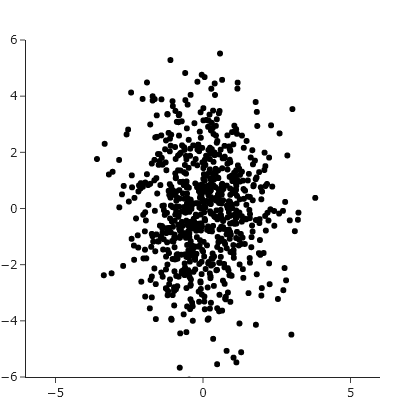
\includegraphics[width=0.35\textwidth]{chapters/mathematical.basis/figures/scaled_cov.png}
	\caption{Uncorrelated scaled variables with different scaling in the $x$ and $y$ axis. \GitChapterOneExamples}
	\label{scaled_cov}
\end{figure}

Lastly, over the scaled data let us follow with a rotation transformation (\autoref{rotated_cov}). Recall that any orthogonal matrix is in fact a rotation matrix, and specifically the rotation matrix of degree $\theta $ in $\R^2$ is given by:
$$R = \left( \begin{array}{ccc}  \cos\theta  & -\sin\theta  \\  \sin\theta  & \cos\theta  \end{array} \right)$$

As we can see in \autoref{rotated_cov} the transformed data shows a correlation between the $x$ and $y$ axes. To understand the reasoning behind let us calculate the sample covariance matrix of the scaled and then rotated data.

$$
\begin{array}{ccl}
	\widehat{\Sigma}_{rotated} & = & =\frac{1}{m-1}\left(RS\X\right)\left(RS\X\right)^{\top}=RS\left(\frac{1}{m-1}\X\X^{\top}\right)\left(RS\right)^{\top}R\left(S\widehat{\Sigma}S^{\top}\right)R^{\top}\\
	\\
	& = & R\left[\begin{array}{cc}
		\left(s_{1}\sigma\right)^{2} & 0\\
		0 & \left(s_{2}\sigma\right)^{2}
	\end{array}\right]R^{\top}=\sigma^{2}\left[\begin{array}{cc}
		s_{1}^{2}\cos^{2}\theta+s_{2}^{2}\sin^{2}\theta\,\, & \sin\theta\cos\theta\left(s_{1}^{2}-s_{2}^{2}\right)\\
		\sin\theta\cos\theta\left(s_{1}^{2}-s_{2}^{2}\right) & s_{1}^{2}\sin^{2}\theta+s_{2}^{2}\cos^{2}\theta
	\end{array}\right]
\end{array}
$$

As the off diagonal element of the covariance matrix is non-zero, the two variables are correlated. Note that if we would not have applied an \emph{asymmetric} scaling (i.e if $s_1=s_2$), the off diagonal elements would have been zero. This means that rotation alone is not sufficient to induce correlations between random variables.

\begin{figure}[h!]
	\centering
	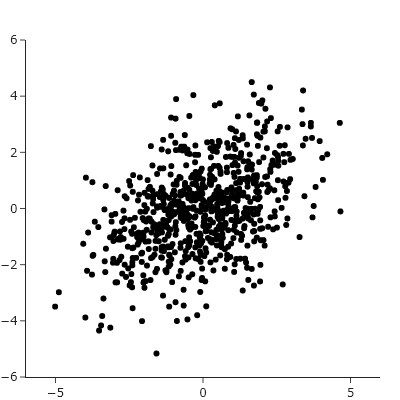
\includegraphics[width=0.35\textwidth]{chapters/mathematical.basis/figures/correlated_cov.png}
	\caption{Correlated variables produced by rotation of uncorrelated variables. \GitChapterOneExamples}
	\label{rotated_cov}
\end{figure}

\begin{remark}
The form obtained above, where we multiply an orthogonal matrix $R$ by a diagonal matrix and then by another orthogonal matrix $R^\top$ is in fact the EVD of the sample covariance matrix of the transformed data. We will return to this point when we discuss the Principal Component Analysis algorithm (\ref{pca}).
\end{remark}



\subsection{Probability Inequalities}
Being able to bound (from below or from above) the probability of different events is an important tool in machine learning. They are used in different senarios such as bounding the errors of a learning algorithm or concluding how good can we expect our algorithm to perform for a given sample size (and how this will change if we increase the sample size). For example, the law of large numbers states that if we take the empirical average (the sample mean) of enough i.i.d. random variables, it will be, most likely, very close to the expected value. Probability inequalities provide us a way to estimate how many samples are "enough".

\begin{example}
Suppose we have a bag containing red and blue balls and we would like to estimate the fraction $p$ of red balls in the bag by randomly picking one ball at a time and then putting it back in. The straightforward strategy is to draw $m$ samples and then to use the following estimation ("prediction")
\[
\widehat{p} =  \frac{1}{m}\sum_{i=1}^{m}x_i =\frac{ ~\text{Number of red balls}}{m}~
\]
where $x_i$ equals 1 if the $i$'th ball came out red and 0 otherwise. 
It is clear that $\E [\widehat{p}] = p$. However, we might not reach this exact value due to the fact that we get only limited information. We are only sampling $m$ balls so we might get ``unlucky`` and end up with a non-representative sample. Although less likely, this can happen even if $m$ is very large, even larger than the total number of balls, because each time we returned the ball to the bag. Thus, typically, we must settle for a certain accuracy - an additive error - that is, we will be happy to know that if we sample more than $m$ times, our estimation,  $\widehat{p}$, is going to be within a distance $\eps>0$ from the real $p$. However, no matter how large $m$ is, there is no absolute guarantee that  $\widehat{p}$ will have that required accuracy.

~\\Since $m$ is finite, there is always a finite chance we sample the same color again and again.  So, at most we can require to have enough confidence, say, with probability of $1-\delta$ where $\delta>0$ is small, that $\hat{p}$ is accurate enough ("accurate enough" defined as within  $\epsilon$ from our target, $p$). And now that we posed a realistic requirement, we can ask how large $m$ should be in order  to satisfy it.
\end{example}

The above example demonstrate the general type of questions we will use probability inequalities for: Given an accuracy parameter $\eps > 0$ and a confidence
parameter $\delta \in \left(0,1\right)$, how many samples are needed to guarantee that with probability of at least $1- \delta$, our estimate is within an additive error of at most $\eps$. That is, we aim at constructing an algorithm (a "learner") whose estimations are probably (with probability at least $1-\delta$) approximately (within additive error of at most $\eps$) correct. We then say that given $m$ samples or more,  our learner's estimation will be  \emph{probably approximately correct (PAC)}. The theoretical framework of PAC will be discussed in details in \autoref{chp:PAC}.

\subsubsection{Markov's and Chebyshev's inequalities}
We now recall Markov's and Chebyshev's inequalities and then apply both inequalities to derive concentration inequalities for averages.
\begin{theorem} \textbf{Markov's inequality:} Let $X$ be a nonnegative random variable (i.e. $Im\left(X\right) \subseteq \R _{\ge 0}$) and deonte the expectation value of $X$ by $\E\left[X\right]$. For any $a>0$: $$ \Prob \left(X \geq a\right) \leq \frac{\E\left[X\right]}{a}$$
\end{theorem}
\begin{proof}
Let $f\left(x\right)$ be the density function of $x$. Since $X$ is non-negative so $f\left(x\right)=0$ for $x<0$. Thus,
\begin{align*}
	\frac{\E\left[X\right]}{a} &= \frac{1}{a}\int_{0} ^\infty f(x) x \,dx \ge \frac{1}{a}\int_{x =a} ^\infty f(x) x \,dx \ge \frac{1}{a}\int_{x =a} ^\infty f(x) a \, dx=\Prob\left(X \ge a\right)
\end{align*}
\end{proof}


\begin{corollary} \label{cor:markovAve}
Let $X_1,\ldots,X_m$ be $m$ i.i.d. non-negative random variables and denote the expectation value of each by  $\E\left[X_i\right]=\E\left[X\right]\,\,\, i = 1,\ldots,m$. Denote also  $\overline{X}=\frac{1}{m} \sum_{i=1} ^m X_i$. Then for any  $a>0$: $$ \Prob \left[\overline{X} \geq a\right] \leq \frac{\E\left[X \right]}{a}$$
\end{corollary}
\begin{proof}
As $\overline{X}$ is a non-negative random variable let us apply Markov's Inequality. So: $\Prob \left(\overline{X} \geq a\right) \leq \E\left[\overline{X}\right]/a$. Now 
\begin{align*}
	\E\left[\overline{X}\right] = \E\left[\frac{1}{m} \sum_{i=1} ^m X_i \right] 
		= \frac{1}{m} \sum_{i=1} ^m \E\left[X_i\right] 
		= \frac{1}{m} \sum_{i=1} ^m \E\left[X\right] 
		= \E\left[X\right]
\end{align*}
and therefore, we obtain the desired bound.
\end{proof}

Markov's inequality gives a bound in terms of the expectation value $\E\left[X\right]$, but it can be used to obtain also a bound in terms of the variance of $X$. This bound is called Chebyshev's inequality and does not require $X$ to be non-negative.  
\begin{theorem} \textbf{Chebyshev's inequality:} For a random variable $X$ with finite mean  $\E\left[X\right]$ and a variance $Var\left(X\right)$ and for every $ a> 0$ $$	\Prob\left[\left|X-\E \left[X\right]\right| \geq a\right] \leq \frac{Var\left(X\right)}{a^2}$$
\end{theorem}
\begin{proof}
Consider the random variable $Y=\left(X-\E\left[X\right]\right)^2$. This is a non-negative random variable and as such we can apply Markov's inequality over it. We obtain that $$\Prob\left[\left(X-\E \left[X\right]\right)^2 \geq a^2\right] \leq \frac{Var\left(X\right)}{a^2}$$
To finish the proof, simply observe that $\Prob\left[\left|X-\E\left[X\right]\right| \geq a\right] = \Prob\left[\left(X-\E\left[X\right]\right)^2 \geq a^2\right]$.
\end{proof}
Unlike in the case of the expectation value, the variance of the average of i.i.d. random variables is not equal to the variance of the original random variable. 
For example, for $m$ i.i.d. random variables, $X_1,\ldots, X_m$, with a variance $Var(X_i)=Var(X)$, $i=1..m$,  we have
\begin{align} \label{eq:varAve}
	V \left[\frac{1}{m} \sum_{i=1} ^m X_i \right] = 
	\frac{1}{m^2} V \left[\sum_{i=1} ^m X_i \right] \notag 
	= \frac{1}{m^2} \sum_{i=1} ^m Var(X_i) \notag 
	= \frac{1}{m^2} \sum_{i=1} ^m Var(X) \notag
	= \frac{1}{m} Var(X)~.
\end{align}
where we used the fact the  $ Var \left[X_1+X_2 \right] = Var\left(X_1\right)+Var\left(X_2\right)$ for independent $X_1$ and $X_2$.
In particular, the variance of the average tends to zero when $m$ tends to infinity. This leads to a much better concentration inequality.
\begin{corollary} \label{cor:chebysevAve}
Let $X_1,\ldots,X_m$ be $m$ i.i.d random variables with a finite variance $Var\left(X\right)$. Denoting $\overline{X}=\frac{1}{m} \sum_{i=1} ^m X_i$. For any $a>0$, it holds that $$\Prob \left[\left|\overline{X}-\E \left[\overline{X}\right]\right| \geq a\right] = \Prob \left[\left|\overline{X}-\E \left[X\right]\right| \geq a\right] \leq \frac{Var\left(X\right)}{m\cdot a^2}$$
\end{corollary}

For a positive integer $k$, the $k$-th \emph{moment} of a random variable $X$ is defined by $\ensuremath{\mathbb{E}}[X^k]$. As we just saw, Markov's inequality exploits only information about the first moment, while Chebyshev's inequality  uses both the first and the second moments. Comparing the bounds in \ref{cor:markovAve} and \ref{cor:chebysevAve}, we see that using both the first and the second moments, we obtain better concentration inequalities than using only the first. We shall see soon that more generally, the more moments we use, the better the bounds we get.

\subsubsection{Coin Prediction Example}  \label{sec:basicConcentration}
Let us consider the problem of estimating the bias of a coin, or in short 'coin prediction'. This will allow us to introduce the important concept of the \textit{sample complexity}, to demonstrate the usefulness and limitations of the Markov's and Chebyshev's inequalities as well as a new one called Hoeffding's inequality.

~\\Formally, a coin flip is a Bernoulli random variable $Z$ which takes the value 1 for "Heads" or 0 for "tails". We shall denote the probability distribution of $Z$ by $\Dc_p$, where $0\le p \le 1$ and $\Dc_p(1)=p, \Dc_p(0)=1-p$ are the probabilities to obtain 1 and 0 correspondingly. Let this be a fair coin where $p=1/2$. Let the following be a sequence of $m$ tosses of this coin $Z_1,\ldots,Z_m\iid Ber\left(p\right)$ and denote the results of the tosses (that is, the samples) by $S = \left(z_1,\ldots, z_m\right)$. Denote the probability of obtaining a specific $S$ by $\Dc _p ^m\left(S\right)$ (or simply by $\Dc ^m\left(S\right)$).


~\\A coin prediction \emph{learning algorithm}, $\Ac$, is a procedure which takes as an input a sequence $S$, drawn according to $\Dc_p ^m$, and produces as an output an estimation of $p$. This estimation, also called ``prediction``, is denoted  by $\Ac\left(S\right)$ or $\widehat{p}\left(S\right)$ or simply $\widehat{p}$. Since $S$ is finite, we do not expect our estimation $\widehat{p}$ to be exact. Instead, we will settle for an algorithm that yields a $\widehat{p}$ which satisfies  $\left|\widehat{p}-p|\right|\le \eps$, for some  $0< \eps <1$ which is called the \emph{accuracy} parameter. Even then, there is always (unless $p$  equals 1 or 0) \textit{some} chance that the drawn sequence would be highly non-representative. For example, it can come out all 0's  in spite of $p$ being close to 1. So it is impossible to obtain a guarantee that $\left|\widehat{p}-p\right|\le\eps$ holds with absolute certainty. 

~\\Hence, we introduce a \emph{confidence} parameter $\delta\in\left(0,1\right)$, and require that the event $\left\{S : \left|\widehat{p}-p\right|>\eps\right\}$ occurs with a probability of at most $\delta$. In other words, we require our algorithm to be such that the probability of flipping the coin $m$ times and obtaining a sequence $S$ that causes it to produce an inaccurate estimation, $\widehat{p}\left(S\right)$ ('inaccurate' meaning $\left|\widehat{p}-p\right|>\eps$ ) is smaller or equal to $\delta$. 

~\\Intuitively, the larger the number of flips, the more information we have about the coin and the better chance we have to satisfy the accuracy and confidence requirements. 
Since the accuracy and confidence parameters $\eps$ and $\delta$ are fixed, there should be some finite number of flips $m_\Ac$ (which depends on  $\eps,\delta$ and $\Ac$) such that for any sample of size $m\ge m_\Ac$ our algorithm satisfies the above accuracy and confidence requirements. If such $m_\Ac$ exists, we say that our algorithm is a \textit{learning algorithm} for the task of coin prediction. Mathematically speaking, we are looking for an algorithm that satisfies the following definition:
    
\begin{definition}  \label{def:sampleCoin}
Let $\Ac$ be an algorithm, which will be also denoted as $\widehat{p}\left(S\right)$ that given a set of coin tosses samples $S\in\left\{0,1\right\}^m$ returns $\widehat{p}\in\left[0,1\right]$ and satisfies the following conditions:\\
\begin{itemize}
\item For any $\eps,\delta\in\left(0,1\right)$, there exists a non-negative integer $m_\Ac\left(\eps,\delta\right)$ such that, if a sequence $S$ of $m$ numbers, where $m\ge m_\Ac$, is generated according to $\Dc ^m_p$,  then,  \textbf{for any $0\le p\le 1$}: $$\Dc ^{m}_p \left[ \left|\widehat{p}\left(S\right)-p\right| > \eps \right] \le  \delta$$
Namely, the probability to get a sample $S$ such that the algorithm's output $\widehat{p}\left(S\right)$ will not be in the interval $\left[p\pm\eps\right]$ is less or equals to $\delta$.\\
\item If a sequence $S$ of $m$ numbers, where $m < m_\Ac$, is generated, \textbf{there exists a $p$}, with $0\le p\le 1$, such that:
		$$ \Dc ^{m}_p \left[ \left|\widehat{p}\left(S\right)-p\right| >  \eps \right] > \delta$$
		
	\end{itemize}
The function $m_\Ac(\eps,\delta)$: $\left[0,1\right]\times \left[0,1\right]\rightarrow \N$ is called the \emph{sample complexity} of the algorithm $\Ac$.
\end{definition}

~\\The first condition means that regardless to the true value of $p$, it is enough to draw $m_\Ac$ samples (i.e., to toss the coin $m_\Ac$ times) in order to know $p$, with a certainty of $1-\delta$ and an accuracy of $\pm \eps$. The second conditions means that, at least for some values of $p$, drawing $m_\Ac\left(\eps,\delta\right)-1$ samples would \textit{not} be enough for that.

~\\Note that the confidence requirement must fold \emph{independently of the procedure by which the coins are provided}. That is, independently of the way $\widehat{p}$ is chosen. It does not matter if, for example, the coin is randomly drawn from a pile of coins where most coins are approximately fair (most of their $p$'s are close to $1/2$) or where most are faked in a specific way, (their $p$'s are concentrated around, say, $\frac{1}{4}$ ),  or where all $p$'s are equally probable.

\paragraph{Choosing an Algorithm}

Let us now look for an algorithm that satisfies the above definition. Given a sample $S=\left(z_1, \ldots, z_m\right)$ the most straightforward estimate of $p$ is the empirical proportion of heads (ones), namely
$$\widehat{p}\left(S\right)=\frac{1}{m} \sum_{i=1} ^m z_m$$
So we have a very simple algorithm for coin prediction, "Count the ones and divide by the number of tosses". Let us show that this algorithm satisfies the definition above.

~\\We begin with noticing that this estimator, being the empirical mean of the parameter is an unbised estimator or $p$. As such it can achieve, for the right sample $S$, that $\left|\widehat{p}-p\right| = 0$. Next, we will test the quality of $\widehat{p}$ as an estimator of $p$. In other words, how many coin flips we need to ensure that $\widehat{p}$ is, most probably, very close to its expectation value, $p$? To answer this question, we can use concentration inequalities.

\paragraph{Estimating Sample Complexity Using Markov's Inequality}

For a direct application of Markov's inequality we take  $|\widehat{p}-p|$ as our random variable. We then need to calculate $\frac{1}{\eps}\E\left[\left|\widehat{p}-p\right|\right]$ and extract its dependence on the sample size $m$. By doing so we achieve the following bound:
$$
\Dc_p ^m \left[\left|\widehat{p}-p\right| \geq \eps \right]  \le \frac{1}{\sqrt{4m\eps^2}}
$$
If we select $m$ to be $$m\ge  \left \lceil \frac{1}{4\eps^2} \cdot \frac{1}{\delta^2} \right \rceil $$
then the right-hand side is smaller or equals to $\delta$. So, for any $\eps,\delta\in\left(0,1\right)$, if we sample $m_\Ac\left(\eps,\delta\right)\geq \left \lceil \frac{1}{4\eps^2} \cdot \frac{1}{\delta^2} \right \rceil $ samples then this learning algorithm achieves that $$ \Dc ^{m}_p \left[ \left|\widehat{p}\left(S\right)-p\right| >  \eps \right] > \delta$$ 


\paragraph{Estimating Sample Complexity Using Chebyshev's Inequality}
To improve the upper bound seen above (i.e find a sample complexity function that will need less samples), let us use Chebyshev's inequality. As the variance of a Bernoulli random variable is $p\left(1-p\right) \le 1/4$, when applying corollary \ref{cor:chebysevAve} we get:
$$ \Dc_p ^m \left[\left|\widehat{p}-p\right| \ge \eps\right] = \Dc_p ^m\left[\left|\widehat{p}-\E\left[\widehat{p}\right]\right| \ge \eps\right] \le \frac{p(1-p)}{m\epsilon^2} \le \frac{1}{4m \eps ^2}$$

We see that the bound obtained using Chebyshev's inequality tends to zero as $\frac{1}{m}$ while the one obtained from Markov's inequality tends to zero as $\frac{1}{\sqrt{m}}$.
This fact enables us to obtain a better bound for the sample complexity:

\begin{corollary}  \label{cor:basicConcentration}
The sample complexity of coin prediction is bounded above by $m\left(\eps,\delta\right) \le \left \lceil \frac{1}{4\epsilon^2} \cdot \frac{1}{\delta} \right \rceil$.
\end{corollary}


\paragraph{Estimating Sample Complexity Using Hoeffding's Inequality}
A natural question which arises is whether the obtained bound is optimal (tight) or there exists an even bound of the sample complexity. 
Indeed, we can further improve the bound by exploiting the fact that our random variable not only has a finite variance, but it is also bounded between $0$ and $1$. For this end we use Hoeffding's inequality for the average of independent and bounded random variables. 

\begin{theorem}[Hoeffding's inequality]
Let $X_1, \ldots X_m$ be independent and bounded random variables with $a_i \leq X_i \leq b_i$. Let $\overline{X} = \frac{1}{m} \sum_{i=1} ^m X_i$. Then,
$$\Prob  \left[ \left|\overline{X} - \E\left[\overline{X}\right]\right| \geq \eps\right] \leq 2 \exp \left( \frac{-2m^2 \epsilon^2}{\sum _{i =1} ^m (b_i-a_i)^2} \right)$$
\end{theorem}

\begin{corollary}
Let $X_1, \ldots X_m$ be a sequence of $m$  i.i.d random variables, each with an expectation value $\E\left[X\right]$ and all of which are bounded: $a \leq X_i \leq b$. Denote $\overline{X} = \frac{1}{m} \sum_{i=1} ^m X_i$ then:$$ Prob  \left[\left|\overline{X} - \E\left[X\right]\right| \geq \eps\right] \leq 2 \exp \left( \frac{-2 m \epsilon^2}{\left(b-a\right)^2} \right)$$
\end{corollary}


By applying Hoeffding's inequality to the case of coin prediction problem, then for a sample of size $m$, we obtain that:
$$ \Dc_p ^m \left[\left|\widehat{p}-p\right| \ge \eps \right]\leq  2 \exp\left(-2 m \eps ^2\right)$$

Therefore, using Hoeffding's Inequality we are able to get a bound which converges exponentially in $m$. By taking $m\ge \left \lceil \frac{1}{2\epsilon^2} \cdot \log(\frac{2}{\delta}) \right \rceil$ samples we obtain that this probability is bound above by $\delta$ as required and conclude that:
\begin{corollary}
The coin prediction algorithm, $\widehat{p}\left(S\right)$, which estimates $p$ by the number of ones (heads) divided by the number of coin flips, is a learning algorithm satisfying definition \autoref{sampleCoin} with a sample complexity which is bounded above by
	$m_\Ac\left(\eps,\delta\right) \le \left \lceil \frac{1}{2\eps^2} \cdot\log(\frac{2}{\delta}) \right \rceil$.
\end{corollary}






